\chapter{DNA transient binding on a gold nanorod: controlled fluorescence enhancement both in space and time}
\label{chapter:transient}
\graphicspath{{./chapters/c5_transient_binding/figures/}}

%============================== MAIN =======================================
\begin{abstract}
  \textbf{Abstract} Fluorescence enhancement by plasmonic nanostructures enable the detection of the dyes with low quantum yield and improves the yield of quantum solid-state light sources.
  Here we demonstrate a DNA based transient binding method to repeatedly and reproducibly study many single molecules by fluorescence enhancement on a single nanorod at the same spot on its tip.
  The heterogeneous excitation and emission enhancement are avoided by looking at the same nanorod and same binding site.
  Bleaching in the plasmonic enhanced single-molecules study is no longer a problem as the bleached molecules can be replaced by new ones.
  The distribution of enhancement factor, binding times and the stability of binding events are characterized.
\end{abstract}

\newpage
\section{Introduction}
Plasmonic nanostructures (nano-antennae) confine light to very small spatial dimensions overcoming the optical diffraction limit enabling detection of single-molecules at millimolar or micromolar concentrations, which is otherwise extremely challenging in conventional microscopy.\cite{levene2003zeromode,punj2013a,schuller2010plasmonics}
These optical nano-antennas strongly interact with quantum emitters altering the emission rates, quantum yield and nonradiative dissipation of the excited state.
Placed at the right distance from these antennae they can enhance the fluorescence of the emitters up to a few orders of magnitude thereby enabling the detection of dyes with poor quantum yield.\cite{lakowicz2005radiative,anger2006enhancement,kinkhabwala2009large,acuna2012fluorescence,yuan2013thousandfold,khatua2014resonant}
The high electric field near the nanorod will lead to excitation enhancement while the high local density of optical states enhances the emission rates of the emitters leading to improvement in the quantum yield.
But close to the metal surface, the nano-structure may also act as an energy sink quenching the fluorescence.\cite{seelig2007nanoparticleinduced,muskens2007strong,acuna2012distance,matsuzaki2017strong}
Emitters will experience different excitation power at different points in space because of the extremely inhomogeneous electric field near the plasmonic structures.
The emission enhancement and quenching are also highly dependent on the distance of the dye from the plasmonic structures.


Different approaches to study single-molecules by fluorescence enhancement may involve free diffusion, non-specific sticking or immobilization of the emitters around the nanostructures, all of which may leads to random positioning of the emitters around the antenna and inhomogeneous excitation and emission.\cite{pradhan2016goldnanorodenhanced,yuan2013thousandfold,zhang2017gold}
Uniform excitation and a better understanding of the photophysics of the fluorescent probes are necessary to fully understand the activity of biological or chemical systems as the light itself can perturb the system under study.
For instance, recently we found that the different excitation field strength in the near field of a gold nanorod leads to different midpoint potential of a redox indicator Methylene Blue and the origin of this change was not clear as we don't precisely control the position of the dye.\cite{zhang2017gold}
Diffusion or immobilization methods pose a limit to the observation time of the single molecules.
Diffusion times in the near-field are often shorter (\SIrange{1}{1000}{\us}) than the characteristic times of biomolecular processes (\SI{>1}{\ms}) making it difficult to study slower processes.
While the molecules can be kept at the same position indefinitely by immobilization, bleaching limits the time a molecule can be observed, which means the molecule stops fluorescing after a while.
This limits the number of single molecules to \textit{one} that can be studied per \textit{one nano-antenna}.


The highly predictable base pairing, binding energy, and length of nucleic acids have allowed the development of a super-resolution technique called DNA-PAINT.\cite{jungmann2010singlemolecule,lin2012submicrometre,schnitzbauer2017superresolution}
The necessary blinking required for super resolution is generated by the transient binding of a short piece of dye-labeled DNA ('imager') to its complementary target ('docking') strands on the structure \textit{in vitro} or \textit{in vivo}.
Here we propose to use the transient binding of DNA to solve both spatial and dynamical uncertainties.
The chemistry and kinetics of ssDNA binding are well understood at single-molecule level and widely available, thanks to the rapid development of DNA-PAINT and DNA based biosensors.\cite{sassolas2008dna,jungmann2010singlemolecule}
The binding time of the imager to the docking strand can be tuned by the electrolyte concentration, number of base pairs, temperature etc. while the length can be controlled by the number of base pairs with a resolution of \SI{0.33}{\nm} per base pair.
As DNA has a persistence length of \SI{\sim50}{\nm}, it can minimize the bending and stabilize the strand around the nanostructure.\cite{manning2006the}


We choose a gold nanorod as the plasmonic nanoantenna in the current study for its simplicity, high tunability of its surface plasmon resonance (SPR) and accessibility of its near field to the bigger molecules like proteins and other biomolecules.
The nanorod can intensify the electric field by two to three orders of magnitude when irradiated with a resonant laser.
The fluorescence enhancement relies on the overlap of the spectrum of the dye with the SPR of the rod and the laser excitation.
The optimum distance for enhancement is \SIrange{3}{5}{\nm}; closer to the rod, fluorescence quenching will dominate; too far away from the rod, the contribution from the excitation enhancement will fade.
For this reason, we choose 10 base pair distance away from the surface which should lead to a distance of \SIrange{3.5}{4}{\nm}.
The number of docking strands on a nanorod is controlled down to one that is responsible for enhancement which is simply done by coating the rest of the surface by a passivating ligand.
We will characterize the controllability of the enhancement factor, binding time, stability of the docking strand on the nanorod.
We will show that a single gold nanorod with the right binding site is enough to study a statistical number of single molecules by fluorescence enhancement.

%====================EXPERIMENTAL SECTION=======================
\section{Methods}
\paragraph*{Materials.} Ethanol (\SI{99.8}{\percent}), methanol (\SI{99.8}{\percent}), 3-Mercaptopropyl)trimethoxysilane(MPTS, \SI{95}{\percent}), cysteamine (\SI{98}{\percent}), thioglycolic acid (\SI{99}{\percent}), Potassium chloride (\ce(KCl)), 4-(2-Hydroxyethyl) piperazine-1-ethanesulfonic acid (HEPES, \SI{99.5}{\percent}), Bovine serum albumin (BSA, \SI{96}{\percent}), Tris(2-carboxyethyl) phosphine hydrochloride (TCEP, \SI{98}{\percent}) were purchased from Sigma-Aldrich; 
Magnesium chloride (\ce{MgCl2}), Hydrogen peroxide (\ce{H2O2}, \SI{30}{\percent}), Sodium acetate (\ce{CH3COONa}, \SI{99}{\percent}), Potassium dihydrogenphosphate (\ce{KH2PO4}), disodium hydrogenphosphate (\ce{Na2HPO4}) from Merck;
Ammonium hydroxide (\ce{NH4OH}, \SI{30}{\percent}), Hydrochloric acid (\ce{HCl}, \SI{37}{\percent}) from Acros Organics;
succinimidyl 4-(p-maleimidophenyl)butyrate (SMPB) from ThermoFisher.
Phosphate buffered saline (PBS) pH 7.4 contained \SI{137}{\mM} \ce{NaCl}, \SI{2.7}{\mM} \ce{KCl}, \SI{10}{\mM} \ce{Na2HPO4} and \SI{1.8}{\mM} \ce{KH2PO4}.
HEPES pH 7 buffer contain \SI{20}{\mM} HEPES. Acetate buffer pH 4 was prepared from \SI{164}{\mM} \ce{CH3COOH} and \SI{36}{\mM} \ce{CH3COONa}.


\paragraph*{Oligonucleotides.} The following DNA oligonucleotides were purchased from Integrated DNA Technologies:
\begin{itemize}
	\item DTPA-5'-ATA CAT CTA GAA ATT-3' (docking strand)
	\item ---Cy5-3'-TAT GTA GAT C-5' (imager strand)
\end{itemize}
Here DTPA represents a hexacyclic group with a dithiol that is used to strongly bind to the gold, Cy5 denotes a red Cyanine dye, and A, T, C, G denotes of DNA bases. 10 bases of docking strand are complementary to ten bases in the imager strand. The chemical structures and the binding scheme is shown in Figure S\ref{SIfig:AuNR-SS_bonding}.


\paragraph*{Silanization of glass surface.} Glass coverslips (Menzel-Glaser, \SI[product-units=repeat]{22x40}{\mm}, no. 1 thickness) were cleaned and activated for silanization before further functionalization.
The coverslips were sonicated in water (\SI{15}{\minute}) and ethanol (\SI{15}{\minute}). 
Then they were heated  at \SI{70}{\celsius} in a bath containing \ce{H2O}/\ce{NH4OH}/\ce{H2O2}(5:1:1) to remove organic impurities on the surface.
This step made the surface very hydrophilic indicating the abundance of hydroxyl and carboxyl functionalities on the surface.
The cover slips were rinsed thoroughly in water and stored in ethanol further use.
To activate the surface, the cover slips were flamed and treated for 30~min in a Teflon incubator with a \SI{1}{\percent} solution of (3-Mercaptopropyl)trimethoxysilane in methanol containing \SI{5}{\percent} glacial acetic acid.
Then the glass slides were rinsed and baked in an oven at \SI{65}{\celsius} for \SI{3}{\hour}.
This results in binding of the silane groups to the active hydroxyl groups and creates a thiol surface that can be used for conjugation with gold nanorods and for passivation of the substrate surface.


\paragraph*{Gold nanorod functionalization.} Gold nanorods (AuNRs) were synthesized using previously published seed-mediated growth in cetyl trimethyl ammonium bromide (CTAB). \cite{nikoobakht2003preparation}
The longitudinal surface plasmon of the AuNRs was \SI{640}{\nm} as obtained from UV-vis spectrum and their average dimensions were $\SI{90}{\nm}\times\SI{45}{\nm}$ as obtained from scanning electron microscopy images.
Excess of CTAB was removed by centrifugation and resuspension in milliQ water.
A thiolated coverslip was mounted in a homemade flow cell.
The AuNR solution was sonicated and immediately incubated in the flow cell for 10~min and then washed with PBS buffer.
This results in around 10 isolated single gold nano-particles per \SI{100}{\um\squared} area on the substrate.
A mixture of \SI{1}{\nM} thiolated docking strand and \SI{10}{\uM} methoxy-poly(ethylene glycol)-thiol (mPEG7-SH, MW 350) in pH 4 buffer was incubated overnight.
mPEG7-SH is used as a the passivating ligand as well as for controlling the number of docking strands on the nanorod.
The ratio between docking strand and passivating molecules was varied to get the desired number of docking strands at the tip of the nanorod.
The length and chemical nature of the passivating ligand were varied to test the flexibility of the docking strand.
Unless mentioned otherwise, the passivating ligand was mPEG.


\paragraph*{Surface passivation.} To prevent the unspecific sticking of imager strands to the surface, the rest of the glass surface was functionalized with bovine serum albumin (BSA).
This was achieved by incubating the coverslips with \SI{1}{mM} succinimidyl 4-(p-maleimidophenyl)butyrate (SMPB), \SI{20}{\uM} BSA and \SI{1}{mM} Tris(2-carboxyethyl)phosphine hydrochloride (TCEP) in HEPES pH 7 for \SI{1}{\hour}.
The succinimidyl group of SMPB binds to the BSA while its maleimide group binds to the thiol on the substrate. 
The unreacted chemicals were washed with PBS pH 7 buffer.


\paragraph*{Imaging and time trace recording.} All the measurements were performed in a home-built confocal microscope that was equipped for Time Correlated Single Photon Counting (TCSPC).
Light from a pulsed picosecond diode laser (Power Technology, Little Rock, AR, USA) with a repetition rate of \SI{40}{\MHz} and a wavelength of \SI{635}{\nm} was passed through a narrow-band clean-up filter (Semrock LD01-640/8-25), then coupled into a single-mode optical fiber.
The output was collimated using a telescope system and reflected by a polychroic mirror (z488/633rpc) onto the back aperture of a high-numerical-aperture oil immersion objective (NA=1.4, Olympus UPLSApo 100x) and then focused to a diffraction limited spot (\SI{300}{\nm}) on the surface of the coverslips.
A power density of \SI[per-mode=repeated-symbol]{100}{\watt\per\cm\squared} was used to image the fluorescent objects on the surface.
Epi-fluorescence from the focal volume was collected through the same objective and focused on a pinhole for spatial filtering, and then passed through an emission filter (z488/635m "dual"-band emission filter, Chroma) to get rid of the laser scattering.
Finally, the fluorescence light was focused onto the active area of an avalanche photodiode (SPCM AQRH-15, Perkin Elmer Inc., USA).
The data was recorded by PicoHarp 300 (PicoQuant GmbH, Berlin, Germany) in time-tagged-time-resolved (t3r) mode which stores both arrival time and micro-time (time after laser excitation) of each photon.


Fluorescence images of the surface of the substrate were acquired by scanning a \SI[product-units=power]{10x10}{\um} area with a step size of \SI{50}{\nm} and a dwell time of \SI{1}{\ms}.
As the nanorods have photoluminiscence lifetimes shorter than the instrument response function (IRF), they are easy to distinguish from the background with longer fluorescence lifetime of the Cy-5 dye (see Figure S\ref{SIfig:trans_int_lt}).
The locations of the nanorods were saved and time traces were recorded for \SI{100}{\s} by parking the laser on the nanorods.
The laser power was \SI[per-mode=repeated-symbol]{10}{\watt\per\cm\squared}, 10 times smaller than the power used for imaging.
The nanorods with the desired number of transient-binding sites (inferred from the number of intensity levels) and fluorescence enhancement factor were selected for further measurements at different experimental conditions and durations.
%=======scheme========
\begin{figure}
	\centering
	\includegraphics[width=\linewidth]{scheme}
	\caption{\textbf{Transient binding schematic:}(left) Nanorods are immobilized on a thiolated glass surface and functionalized with docking strands and mPEG7-SH.
	The rest of the surface is passivated with BSA to prevent non-specific interaction.
	The imager-Cy5 strands in the solution  are shown with a gray dot on one end representing a weaker signal.
	One of the imagers is bound to the docking strand at the tip of the nanorod and is shown with a bright red spot representing fluorescence enhancement.
	(right) Reversible transient binding on the docking sites on a nanorod. The docking strand at the tip of the nanorod gives rise to enhancement while the one on the side of the rod exhibits no enhancement.}
  	\label{sch_trans:setup}
\end{figure}


\section{Results and Discussion}
%========one vs many binding sites========
\paragraph*{Number of binding sites.} The average number of docking strands on a gold nanorod is controlled simply by changing the ratio between the docking DNA and mPEG7-SH.
Figure \ref{fig:timetrace1vsmany}(a) shows the time trace of transient binding on a gold nanorod with the ratio between docking and passivating strand maintained at 1:2000 and Figure \ref{fig:timetrace1vsmany}(c) at a ratio of 1:10000.
The concentration of imager strand was \SI{100}{\nM} with \SI{500}{\mM} \ce{NaCl} in PBS pH 7.4 buffer.
At ratio 1:2000, intensity bursts with different heights were observed and almost $5$ different peak heights can be distinguished from the intensity histogram with the maximum count rate at \SI{120}{ kcps} indicating an enhancement factor of $\sim60$ taking the count rate of un-enhanced imager as \SI{2} { kcps} (SI Fig S\ref{SIfig:timetrace_only_Cy5}).
The different peak heights are shown by the dashed lines and the numberings are done in increasing order of count rates.
The highest intensity shown by the arrow has two step-wise intensity changes resulting from two binding events occurring during the same time.
At ratio 1:10000, two intensity levels can be clearly distinguished both from the time trace and intensity histogram with the maximum enhancement factor of $\sim10$.
The laser power was chosen in a way to detect bursts with fluorescence enhancement down to a factor of two.
\begin{figure}[ht]
	\centering
	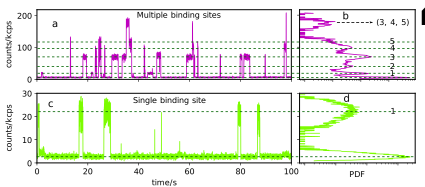
\includegraphics[width=\textwidth]{timetrace1vsmany}%width=\textwidth
	\caption{Time traces of transient binding of \SI{100}{\nM} imager with the docking sites on a gold nanorod with ratios between docking and passivating ligands of 1:2000 (a) and of 1:10000(c).
	The corresponding intensity histograms are shown on the right (b, d).
	The dashed lines connect the peaks in the histogram to the intensity levels in the time trace and the numberings are done in increasing order of the intensities.
	The $(3, 4, 5)_2$ represents the combination of any two arbitrary levels inside the bracket. 
	}
  	\label{fig:timetrace1vsmany}
\end{figure}

\paragraph*{} The gold nanorods were completely functionalized with mPEG7-SH and docking strands by overnight incubation.
Hinterwirth et al. showed that the coverage of \ce{PEG_7} on gold nanoparticles is \SI{4.29}{\per\nm\squared} and the packing density is mostly dependent on the steric hindrance rather than the chemical nature of the ligand.\cite{hinterwirth2013quantifying}
$5.5\times10^4$ chains should be bound to the nanorod with dimension \SI[product-units=repeat]{90x45}{\nm} assuming similar affinity of the passivating ligands and the docking strands.
At ratio 1:2000 between docking and mPEG7, out of ${\sim}27$ docking strands on the gold nanorod, ${\sim}5$ docking sites are observed through the fluorescence enhancement of imager by the gold nanorod.
Similarly at 1:10000 ratio between docking and mPEG7 ${\sim}1$ docking site is observed out of ${\sim}5$ docking strand on the nanorod.
The ratio-metric study at two concentrations shows that ${\sim}1/5^{th}$  of the attached docking strands show fluorescence enhancement.
Assuming uniform distribution of docking strands on the nanorod surface, the effective area on the nanorod for fluorescence enhancement can be calculated as ${\sim}1/5^{th}$ of its total area.
The major contribution to the enhancement comes from the excitation enhancement due to the high intensity of the electric field at the tip of the nanorod that results from the surface plasmon resonance.
Thus we find that the area at its spherical tip within a solid angle of \SI{\sim1.6}{$\pi$} provides for an enhancement of Cy5 at least by a factor of two.
This effective area will vary depending on the SPR of the rod, spectral overlap of the spectrum of the dye with the SPR and laser, the quantum yield of the dye, and the distance of the dye to the surface of the rod.


One of the motivations for the present study is to observe the enhancement over and over again for the same binding site.
Figure S\ref{SIfig:bleaching_free_longtrace} shows transient binding on three different gold nanorods with different enhancement factors.
The two peaks in the intensity histogram of each rod and the absence of multi-step intensity bursts indicate that there is only one distinguishable docking strand.
And the uniform binding and unbinding of imager strands on a particular nanorod over a time scale of \SI{1000}{\s} indicates that there is little variation in DNA binding over time.
However, the frequency of binding and unbinding varied from nanorod to nanorod even for rods with a similar enhancement factor (Fig S\ref{SIfig:bleaching_free_longtrace}A, C).
This can be attributed to the different local environments in the PEG brush around nanorod which can hinder the approach of the imager strand to the docking strand.
When letting the experiment run long enough(\SI{\sim1}{\hour}), it was observed that the intensity bursts completely disappears (Fig. S\ref{SIfig:dissociation_transbind}).
Deliberately applying high laser power also made the transient binding disappear, but also some unequal short bursts appeared.
Goodman et. al.\cite{goodman2016understanding} showed that pulsed laser or high power continuous wave (CW) laser cleave Au-S bonds and two orders magnitude of higher CW laser power is required to have a similar release of Au-S-DNA as achieved by pulsed laser.
The appearance of short and uncontrolled bursts with high pulsed laser was probably non-specific sticking of imager to the rod after the PEG and docking strands dissociated.
While this dissociation can be useful for controlled release in drug delivery, it acts as a disadvantage for the transient binding where we wish to keep the docking permanently attached.
However, the dissociation of the docking strand from the gold can be delayed by using a CW laser instead of a pulsed laser as employed in the current study.

%========Cysteamine vs peg========
\paragraph*{Flexibility of the docking strand.} Different passivating ligands have been tested to understand their effect on the binding kinetics of the imager on the docking strands.
Two short linkers (less than \SI{1}{\nm} length) cysteamine with a basic head group (negative charge) and thioglycolic acid with a positive head group were compared with the longer linker mPEG7-SH (\SI{\sim3.5}{\nm} length).
A transient-binding trace of a cysteamine functionalized and of a PEG-functionalized nanorod can be seen in Figure \ref{fig:timetraceCysvsPeg}.
The intensity bursts for the cysteamine-functionalized nanorod are much noisier than the bursts of the PEG-functionalized nanorod.
The dynamics of the bound imager can be better characterized by the autocorrelation function which is given by $G(\tau)=<I(t)I(t+\tau)>/<I(t)>^2$ and keeps track of the temporal fluctuations of the fluorescence intensity $I(t)$ (where $\tau$ is the lag time and $<...>$ represents time averaging).
The autocorrelation function was calculated for each of the intensity bursts and finally averaged over all the bursts on a time trace.
Figure \ref{fig:timetraceCysvsPeg}(C) shows autocorrelation functions for  PEG (green), cysteamine (magenta) and thioglycol (red) functionalization.
The autocorrelation of cysteamine and thioglycol-functionalization shows two exponential components while the autocorrelation for PEG shows a single exponential decay.
\begin{figure}[ht]
	\centering
	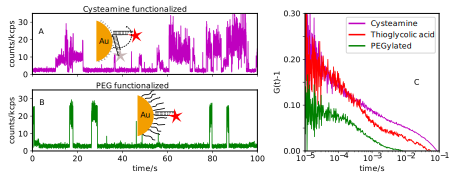
\includegraphics[width=\textwidth]{timetraceCysvsPeg}
	\caption{\textbf{Flexibility of the docking strand:} Time trace of transient binding on a gold nanorod with cysteamine (\ce{C2H7NS})(A) as passivating ligand and mPEG7-SH (B) as passivating ligand.
	Notice the noisier intensity bursts in the case of cysteamine while the bursts for the PEGylated nanorod are quite stable.
	(C) Autocorrelation of intensity bursts for PEG (green), cysteamine (magenta) and thioglycol (red) functionalization.
	Autocorrelation values were obtained by averaging all the individual autocorrelations from each burst on a time trace. 
	Cysteamine and thioglycol have shorter chain lengths but opposite charges of their head group while PEG has longer chain length.
	Inside the time trace plots, the length of the docking strand is compared with length of passivating ligands and possible bending of docking strand resulting in quenching is shown with the colored stars.}
  	\label{fig:timetraceCysvsPeg}
\end{figure}


The decay at shorter time scales (\SI{<1}{\ms}) present in all the three cases is attributed to the cis-trans conformational dynamics of Cy5.\cite{yeh2008tunable}
The Cy5 has a double bond that can undergo cis-trans isomerization (Fig. S\ref{SIfig:AuNR-SS_bonding}) making it planer in the trans form which results in a fluorescent state, whereas in the cis form the conjugated rings go out of plane making the Cy5 molecule non-fluorescent.
The decay at longer time scales (\SI{\sim100}{\ms}) for cysteamine and thioglycol functionalization can be attributed either to the interaction of the docking strand with the functionalized nanorod surface or to free wiggling of the docking strand.
Although the movement happens in nanometer scale, it can be clearly observed because of the strong dependence of the enhancement on the position with respect to the tip of the nanorod.
As the docking strand wiggles, it can come close to the surface of the nanorod resulting in quenching or it can move away from the surface of the tip resulting in enhancement.
The persistence length of DNA\cite{manning2006the} is \SI{50}{\nm} which means the bending is probably coming from the point between the docking oligonucleotide and the gold surface.
However, for a PEG-functionalized nanorod, the longer component is missing indicating the absence of wiggling and more rigidity for the hybridized DNA.
The long PEG chain is providing steric hindrance to the docking strand keeping it straight and away from the gold surface preventing the fluorescence quenching.
Although the PEG brush leads to steric hindrance, apparently the imager strands can still migrate into the brush and bind to the docking strand without compromising the transient binding.


%=======countrate vs duration==========
\paragraph*{Binding time.}
The binding time of the imager to the docking strand depends on many factors: the number of base pairs involved in the binding, the salt concentration, the temperature etc.
For the current study, the number of base pairs involved in the binding was fixed to $10$ and all of the measurements were performed at \SI{500}{\mM} \ce{NaCl} and at room temperature (\SI{298}{\kelvin}).
The length of the imager strand was chosen to be $10$ base pairs to get maximum fluorescence enhancement.
Khatua et. al. obtained maximum fluorescence enhancement at a distance of \SIrange{3}{5}{\nm} from the tip of the gold nanorod for a low quantum yield dye like Crystal Violet.\cite{khatua2014resonant}
10 base pairs of DNA along with the linkers used to attach to the gold as well as the dye results in a length of \SI{\sim4}{\nm} which should result in optimum enhancement.
The binding times of the imager observed from the time traces are shown against the intensity of the bursts in a scatter plot in Figure \ref{fig:countrate_vs_duration}(A).
At lower count rates, more points can be found with longer dwell time, while at higher count rates, most of the bursts have short dwell time. 
The average duration clearly declines after a count rate of \SI{\sim25}{kcps}.
The histogram of binding times of intensity bursts with count rate less than \SI{\sim25}{kcps} is shown in Figure \ref{fig:countrate_vs_duration}(B) which seems to be following an exponential decay with an average value of \SI{1.13}{\s}.
\begin{figure}[ht]
	\centering
	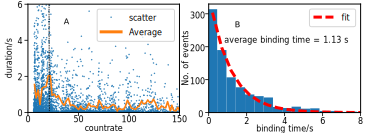
\includegraphics[width=\textwidth]{countrate_vs_duration_nophtns}
	\caption{\textbf{Binding time:} (A)Binding time as a function of the count rate of the intensity bursts of transient binding events.
	It shows the running average of data points obtained from $24$ nanorods with 1 to 5 docking sites on each of them and the shaded area shows the standard deviation.
	The dotted line shows the count rate above which the bleaching starts.
	(B) Histogram of binding times of intensity bursts with count rates smaller than \SI{25}{ kcps}.
	The threshold was selected not to over sample the bleaching events that appear at shorter binding times.
	The average binding time was \SI{1.13}{\s}.}
  	\label{fig:countrate_vs_duration}
\end{figure}

A fluorescent dye normally has an average limit to the total number of photons that it can emit in a particular environment because of bleaching.
Below the count rate of \SI{\sim25}{kcps}, the true binding time of the imager can be observed.
Above \SI{\sim25}{kcps}, the dye bleaches before the imager strand unbinds from the docking strand which results in shortening of the duration of the intensity bursts.
This led to the selection of a threshold maximum of \SI{\sim25}{kcps} for estimating the real binding kinetics; otherwise, the shorter-binding times would be oversampled.
The average binding time of \SI{1.13}{\s} for 10 base pair binding at \SI{500}{\mM} \ce{NaCl} is shorter than the value of \SI{5}{\s} obtained previously.\cite{jungmann2010singlemolecule}
As the docking strand is surrounded by PEG brush, all the 10 bases on the docking strand might not be accessible for binding with the imager which can result in the shortening of the binding time. 

%========Enhancement statistics=========
\paragraph*{Enhancement distribution.}
Considering the strongly inhomogeneous near field of the nanoantenna, we expect a distribution in the enhancement factor.
Figure \ref{fig:int_lt_distribution}(A) shows the distribution of intensities bursts obtained from $24$ nanorods with 1 to 5 observable binding sites with an average count rate of \SI{53}{kcps} corresponding to an enhancement factor of $\sim25$.
The possible positions of the dye at the tip of nanorod are shown in Figure \ref{fig:int_lt_distribution}.
The color map shows the electric field intensity simulated by finite difference time domain(FDTD) in COMSOL.
The lifetime histogram of enhanced fluorescence is shown in magenta (Figure \ref{fig:int_lt_distribution}(C)) while that of un-enhanced fluorescence (in absence of intensity bursts) is shown in green.
The lifetime of un-enhanced Cy5 is \SI{1.8}{\ns} while the lifetime histogram of enhanced bursts is found to be same as the IRF.
\begin{figure}[ht]
	\centering
	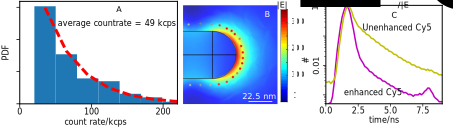
\includegraphics[width=\textwidth]{lifetime_scatplot}
	\caption{Enhancement statistics.(A) Histogram of count rates of intensity bursts of transient binding obtained from $24$ gold nanorods with 1 to 5 docking sites on each of them.
	The average count rate was \SI{53}{ kcps} with an enhancement factor of $\sim 25$.
	(B) Electric field map of the nanorod and the stars symbolizes the positions the dye can occupy at the surface of the nanorod.
	The color bar is the normalized intensity.
	The enhanced dye at the tip are shown in red stars and the unenhanced or quenched dyes at the side of the rod are shown in gray stars.
	(C) Lifetime histogram of all the intensity bursts found in Figure \ref{fig:timetrace1vsmany}(a) shown in magenta while the lifetime histogram of the un-enhanced fluorescence is shown in green.
	}
  	\label{fig:int_lt_distribution}
\end{figure}

As the docking strands are functionalized randomly on the nanorod without specificity to the tip, all the possible enhancement factors are expected with a condition that they should be confined to a small volume at a constant distance from the surface.
A maximum enhancement factor of 100 is observed which is reasonable for a dye with a high quantum yield of \SI{30}{\percent} and a gold nanorod with an intensity maximum of \SI{\sim300}{times} the excitation laser.
The previous study shows that the high intensity near the nanorod can enhance the fluorescence by hundred times which is called excitation enhancement.
For the dye (Crystal violet) with low quantum yield (\SI{1}{\percent}), they observed an emission enhancement by one order of magnitude.
Emission enhancement highly depends on the quantum yield of the dye, poorer the quantum yield better the emission enhancement will be.
For Cy5 with a high quantum yield, no significant emission enhancement is expected, excitation enhancement being the only contributor to the enhancement of the fluorescence intensity.
The most intense bursts come from close to the center of the tip while weak bursts originate from the side.
The histogram of the bursts height should be same as the distribution of light intensity at a distance of around \SI{4}{\nm} from the tip of the nanorod.
The lifetime below IRF shows that the radiative and non-radiative rate is enhanced at least a factor of 10 (lifetime of Cy5 away from the nanorod is \SI{1.8}{\ns}), however, it is not possible to distinguish the two contribution from the current data.
The previous study\cite{seelig2007nanoparticleinduced} shows that even at a distance of \SI{15}{\nm}, the lifetime is already reduced by a factor of 10.
As in the current study, the distance of the dye is just \SI{4}{\nm}, we expect a much shorter lifetime which requires a high-resolution TCSPC to be measurable.
As we don't expect much enhancement in the quantum yield of Cy5, quenching is probably a main contribution to the shortening of the lifetime.

\section{Conclusion}
We demonstrated the observation of many single-molecules with equal enhancement factors on a single gold nanorod with a single binding site.
Different nanorods showed different enhancement factors because of the variation in the position of the docking strand and in the SPR of the nanorod.
But once a nanorod is identified with the desired enhancement factor, as many single-molecules can be studied with the same excitation and emission yields.
The effort to find the best enhancement factor can be reduced by specifically attaching the docking strand at the tip of the rod.
The similar method can be applied to different kind of plasmonic nanostructures and the position of the emitter can be controlled by properly engineering the DNA.
Similarly, different biomolecules and quantum emitters can be studied by attaching them to the imager strand.
%============================== END MAIN =======================================
%=========================== SUPPORTING INFORMATION ==========================
\graphicspath{{chapters/c5_transient_binding/si-figures/}}
%============================ MAIN ==========================
\section{Supporting info}
\begin{figure}[ht]
  \centering
  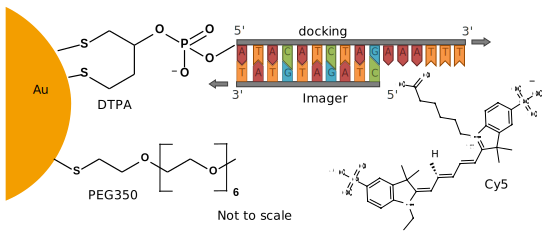
\includegraphics[width=0.8\textwidth]{AuNR-SS_bonding}
  \makeatletter
  \renewcommand{\fnum@figure}{\figurename~S\thefigure}
  \makeatother
  \caption{\textbf{Binding to gold surface} The chemical structures of different components in the transient binding scheme.
  The docking strand is attached to the nanorod through DTPA, which has two thiols attached to the gold atoms.
  The sequence of the docking and the imager strand are shown with their complementary binding.
  The imager strand is labeled with Cy5 at its 5' end.
  The rest of the nanorod surface is functionalized with PEG350, which has 9 monomers giving it a length of \SI{\sim3}{\nm}.}
  \label{SIfig:AuNR-SS_bonding}
\end{figure}

\begin{figure}[ht]
  \centering
  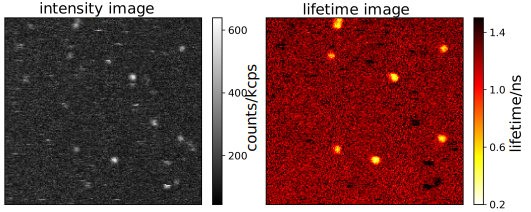
\includegraphics[width=0.8\textwidth]{trans_int_lt_img}
  \makeatletter
  \renewcommand{\fnum@figure}{\figurename~S\thefigure}
  \makeatother
  \caption{A \SI[product-units=power]{10x10}{\um} scanning image of the surface of the substrate with gold nanorod functionalized with docking strand and mPEG7-SH.
  The solution contains \SI{100}{\nM} imager strand in PBS pH 7.4 buffer with \SI{500}{\mM} \ce{NaCl}.
  The image on the left shows counts per millisecond while the image on the right shows the lifetime.
  The spots on the lifetime image correspond to the gold nanorods as they have a much shorter lifetime than the instrument response function.}
  \label{SIfig:trans_int_lt}
\end{figure}
% \subsection*{Replenish and recyacle}
\begin{figure}[ht]
  \centering
  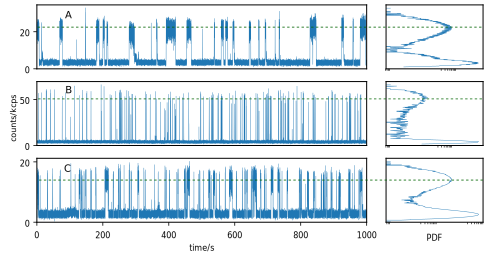
\includegraphics[width=\textwidth]{bleaching_free_longtrace}
  \makeatletter
  \renewcommand{\fnum@figure}{\figurename~S\thefigure}
  \makeatother
  \caption{\textbf{Many single molecules bind to the same binding spot on the same nanorod.} Time traces of three different nanorods, each of them with a single binding site, but with different enhancement factors.
  The histogram of intensities for each time trace is shown on the right and the two peaks indicate the presence of only one observable docking strand.
  Notice the different binding kinetics of trace A and trace C although they have similar enhancement factors.}
  \label{SIfig:bleaching_free_longtrace}
\end{figure}

\begin{figure}[ht]
  \centering
  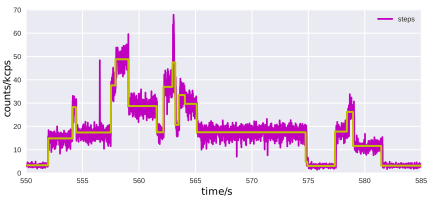
\includegraphics[width=\textwidth]{step_timetrace}
  \makeatletter
  \renewcommand{\fnum@figure}{\figurename~S\thefigure}
  \makeatother
  \caption{\textbf{Multi-step transient binding:}Time trace on a functionalized gold nanorod with multiple transient binding events appearing on top of each other.
  The association and dissociation of each imager strand can be distinguished from the step height and the time of appearance. }
  \label{SIfig: step_transbind}
\end{figure}

% \subsection*{Transient binding on substrate}
\begin{figure}[ht]
  \centering
  \includegraphics[width=\textwidth]{timetrace_only_Cy5}
  \makeatletter
  \renewcommand{\fnum@figure}{\figurename~S\thefigure}
  \makeatother
  \caption{\textbf{Transient binding without nanorod:} (A) Schematic of the transient binding.
  The docking strand was immobilized on the surface through neutravidin and biotin bonding.
  The solution contained \SI{100}{\nM} imager-Cy5 in PBS pH 7.4 buffer.
  Scanning image  in the absense (B) and presence (C) of docking strand on the surface showing the specificity of binding of the imager to the docking strand.
  (D) Time trace of transient binding on a single neutravidin-docking site at \SI{\sim 0.1}{\kW\per\cm\squared} power density, 10 times higher than the laser power used for measurement on the nanorod. The burst heights are \SI{\sim 20}{ kcps} corresponding to single imager-Cy5.
  To compare with the bursts from nanorods and calculate the enhancement factor, the count rate can be divided by 10 to match the laser power on the nanorod as the intensity varies linearly at such low powers.
  A count rate of \SI{2}{ kcps} for unenhanced Cy5 has been used in the main text. 
  }
  \label{SIfig:timetrace_only_Cy5}
\end{figure}
% \subsection*{Dissociation of docking strand}
\begin{figure}[ht]
  \centering
  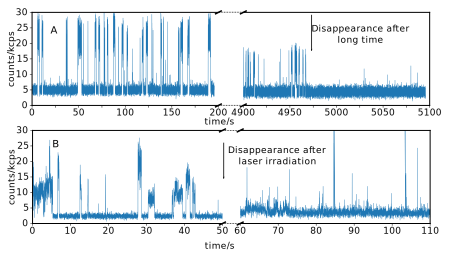
\includegraphics[width=\textwidth]{dissociation_transbind}
  \makeatletter
  \renewcommand{\fnum@figure}{\figurename~S\thefigure}
  \makeatother
  \caption{\textbf{Dissociation of docking strand.}
  (A) The time trace on the top is recorded on a gold nanorod until no docking events any more are observed.
  The transient binding events never reappeared, even after re-flushing with imager strand and realigning the laser focus.
  (B) The transient binding trace on a gold nanrod before and after irradiation with high laser power (\SI[per-mode=repeated-symbol]{1000}{\watt\per\cm\squared}, \SI{40}{\MHz}).
  }
  \label{SIfig:dissociation_transbind}
\end{figure}
% \references{chapters/c4_azurin_sm/azurin}